\section{Boat user control}

\begin{wrapfigure}{l}{0.5\textwidth}
    \label{img:boat_scr}
    \vspace{-20pt}
    \begin{center}
        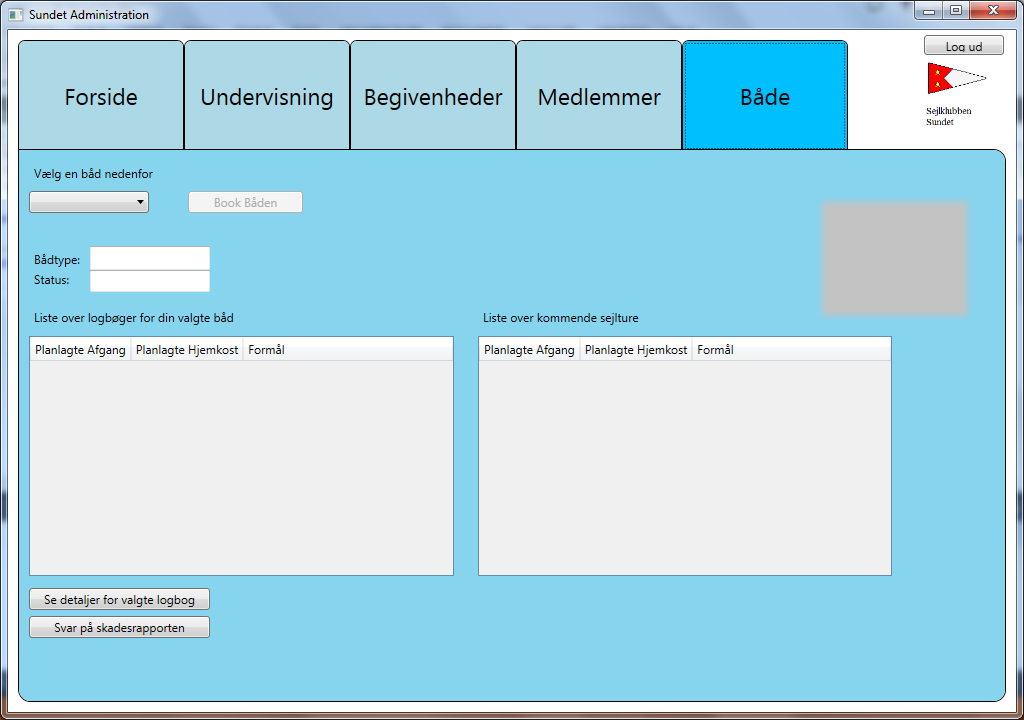
\includegraphics[width=0.48\textwidth]{/Screenshots/boat_scr.png}
    \end{center}
    \vspace{-20pt}
    \caption{Boat screenshot}
    \vspace{-10pt}
\end{wrapfigure}

\textbf{Formål:}

Under Boat kan man få et overblik over hvilke både som der er til rådighed i sejlklubben inklusiv bådtype og status på båden (om den f.eks. er operationel). 
Man kan også booke en båd, se liste over logbøger for en valgt båd og ligeledes se en liste over kommende sejlture (bookings). 

\textbf{Brugergrænseflade:}

På siden findes der flere forskellige controls.
Man starter først med en dropdown menu, hvor man kan vælge hvilken båd man vil se informationer om.
Til højre for den er der en knap ``Book Båden'', som man kan trykke på, hvis man vil booke båden. Når den trykkes på, så åbner der en ny fane, hvor man kan angive bookingsinformation. 
Helt ude til højre er der et billede af hver enkelt båd. 
Under dropdown menuen bliver der vist i en textbox bådtypen og bådens status. 
Til visning af logbøger og kommende sejlture, er der to listbokse ved siden af hinanden, hvor hhv. logbøger og kommende sejlture vises efter dato. 
I selve listboksene kan man se ``Planlagte afgang'', ``Planlagte hjemkomst'' og ``Formål'', ved både logbøger og kommende sejlture. 
Til sidst er der to knapper; ``Se detaljer for valgte logbøger'' og, hvis man er logget ind som administrator, ``Svar på skadesrapporten''. Ved at først vælge en logbog, i listen over logbøger, og derefter klikke på ``Se detaljer for valgte logbøger'', så kan man se detaljer omkring den valgte logbog. 
Hvis der dobbeltklikkes på en logbog i listboksen, så opnår man samme effekt. 
Hvis man er logget ind som administrator, så man kan vælge en logbog, og trykke på ``Svar på skadesrapporten'', hvor der åbnes et nyt vindue, hvor der kan svares på skadesrapporten. 

\textbf{Code-behind:}

Metoden BoatComboBox\_OnSelectionChanged aktiveres ved at vælge en båd i dropdown menuen. 
Hvis der ikke er valgt en båd, så er Book Button (``Booking'') ikke aktiv. 

Først noget hentning af data fra dal og sortering\fxnote{Skal skrives når database oprettes}

Efter dataet er hentet fra \textbf{databasen}, så tjekkes der, at hvis brugeren ikke er supportmedlem, så er BookButton (``Booking'') aktiv. 

Derefter laves der et tjek på om ImagePath er null, hvis ikke, så er billedestien ImagePath, så hver båd har sit eget billede. 
Hvis ImagePath er null, så bliver der vist et gråt billede.

Derefter tjekkes der om båden er operationel og bådtypen hentes og vises i hver deres textbox. 

Til sidst så bliver dataet som hentes fra \textbf{databasen} afbildet i hvert sit datagrid.

